% Figure: Oxidative Stress Vicious Cycle in ME/CFS
% Imbalance creates self-perpetuating damage cascade

\begin{figure}[htbp]
\centering
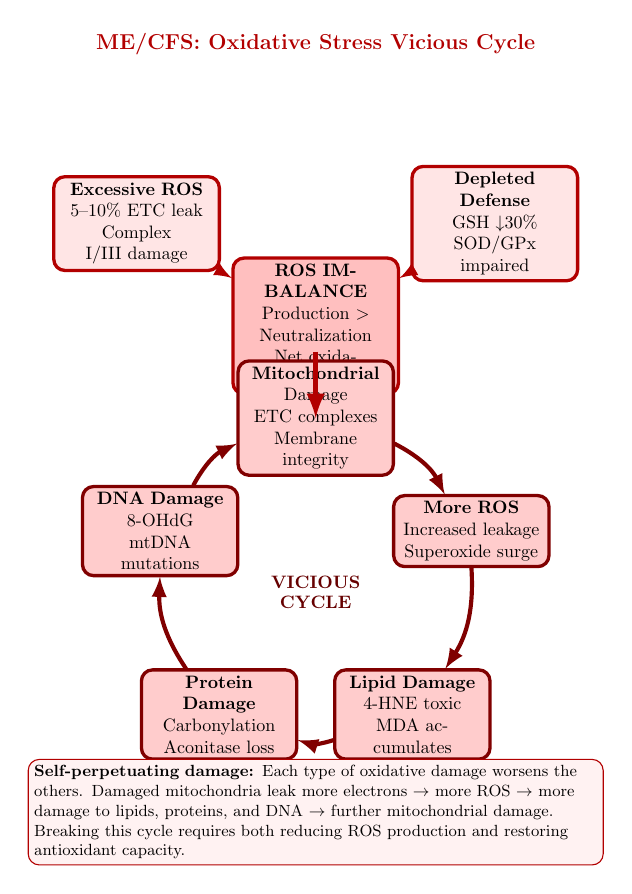
\begin{tikzpicture}[scale=0.65, every node/.style={scale=0.65},
    % Styles
    impaired/.style={draw=red!70!black, fill=red!10, very thick, rounded corners, text width=3cm, align=center, minimum height=1cm},
    pathological/.style={draw=red!50!black, fill=red!20, very thick, rounded corners, text width=2.8cm, align=center, minimum height=1cm},
    impaired-arrow/.style={-latex, very thick, red!70!black},
    cycle-arrow/.style={-latex, ultra thick, red!50!black, line width=1.5pt},
    note/.style={font=\scriptsize\itshape, text width=2.5cm, align=center},
]

% Title
\node[font=\large\bfseries, red!70!black] at (0, 8.5) {ME/CFS: Oxidative Stress Vicious Cycle};

% TOP: Imbalance
\begin{scope}[yshift=5cm]
    % Excessive ROS (left)
    \node[impaired] (ros) at (-3.5, 0) {\textbf{Excessive ROS}\\5--10\% ETC leak\\Complex I/III damage};

    % Depleted antioxidants (right)
    \node[impaired] (antioxidants) at (3.5, 0) {\textbf{Depleted Defense}\\GSH $\downarrow$30\%\\SOD/GPx impaired};

    % Imbalance
    \node[impaired, fill=red!25] (imbalance) at (0, -2) {\textbf{ROS IMBALANCE}\\Production $>$ Neutralization\\Net oxidative damage};

    \draw[impaired-arrow] (ros) -- (imbalance);
    \draw[impaired-arrow] (antioxidants) -- (imbalance);
\end{scope}

% BOTTOM: Vicious cycle
\begin{scope}[yshift=-2cm]
    \def\radius{3.2}
    \def\centerx{0}
    \def\centery{0}

    % Node 1: Mitochondrial damage (top)
    \node[pathological] (mito) at (\centerx, \centery + \radius)
        {\textbf{Mitochondrial}\\Damage\\ETC complexes\\Membrane integrity};

    % Node 2: Increased ROS (right)
    \node[pathological] (ros-up) at (\centerx + \radius*0.95, \centery + \radius*0.31)
        {\textbf{More ROS}\\Increased leakage\\Superoxide surge};

    % Node 3: Lipid peroxidation (bottom right)
    \node[pathological] (lipid) at (\centerx + \radius*0.59, \centery - \radius*0.81)
        {\textbf{Lipid Damage}\\4-HNE toxic\\MDA accumulates};

    % Node 4: Protein damage (bottom left)
    \node[pathological] (protein) at (\centerx - \radius*0.59, \centery - \radius*0.81)
        {\textbf{Protein Damage}\\Carbonylation\\Aconitase loss};

    % Node 5: DNA damage (left)
    \node[pathological] (dna) at (\centerx - \radius*0.95, \centery + \radius*0.31)
        {\textbf{DNA Damage}\\8-OHdG\\mtDNA mutations};

    % Cycle arrows (clockwise)
    \draw[cycle-arrow, bend left=18] (mito) to (ros-up);
    \draw[cycle-arrow, bend left=18] (ros-up) to (lipid);
    \draw[cycle-arrow, bend left=18] (lipid) to (protein);
    \draw[cycle-arrow, bend left=18] (protein) to (dna);
    \draw[cycle-arrow, bend left=18] (dna) to (mito);

    % Central label
    \node[font=\bfseries, red!40!black] at (\centerx, \centery) {VICIOUS};
    \node[font=\bfseries, red!40!black] at (\centerx, \centery - 0.4) {CYCLE};
\end{scope}

% Arrow from imbalance to cycle
\draw[impaired-arrow, line width=2pt] (0, 2.5) -- (0, 1.2);

% Key point box
\node[draw=red!70!black, fill=red!5, rounded corners, text width=11cm, align=left, font=\small] at (0, -6.5) {
\textbf{Self-perpetuating damage:} Each type of oxidative damage worsens the others. Damaged mitochondria leak more electrons $\rightarrow$ more ROS $\rightarrow$ more damage to lipids, proteins, and DNA $\rightarrow$ further mitochondrial damage. Breaking this cycle requires both reducing ROS production and restoring antioxidant capacity.
};

\end{tikzpicture}
\caption{ME/CFS oxidative stress vicious cycle with self-perpetuating damage.}
\label{fig:oxidative-stress-mecfs}
\end{figure}
